\chapter{Introduction}\label{intro}

\section{Overview}

Cancer is a genetic disease that has been one of the leading causes of deaths globally for many years \citep{Bray2021TheWorldwide}. Cancer development, or carcinogenesis, occurs as a consequence of changes in the normal cells that stimulate cell proliferation \citep{Weinberg1996HowArises}. The resulting tumours can damage the healthy part of the local tissues by invasion, increased infection, interference with the organ function and so on \citep{Tobias2014CancerManagement}. There are roughly 100 cancers making up the major types: \gls{carcinoma}, \gls{lymphoma}, \gls{leukaemia}, \gls{sarcoma} and \gls{neuroectodermal_tumour}. Cancer treatment relies on our understanding of the specific cancer sample. For instance, trastuzumab, which targets the HER2 protein, is known to deliver good response in HER2-positive, but poor response in HER2-negative breast cancers \citep{Kreutzfeldt2020TheTherapies}. Another key to cancer treatment is early diagnosis \citep{Hawkes2019CancerDiagnosis}. For example, the 5-year survival rate for prostate cancer is 100\% \textit{v.s.} 48\% if intervened at stage 1 and 4, respectively. 

The process of \gls{carcinogenesis} is characterised by mutations \citep{Stratton2009}. Whether a mutation occurs is in turn determined by whether mutagens can form a \gls{lesion} in the DNA and whether the repair systems can correctly fix the lesion \citep{Chatterjee2017MechanismsMutagenesis}. While every cancer sample is different in terms of mutations, certain mutation patterns have been associated with certain cancer types \citep{Alexandrov2013,Polak2015,Campbell2020}. Since all cancers originate from a normal cell \citep{Hanahan2011HallmarksGeneration}, different patterns of cancer \gls{mutagenesis} may reflect the mutation tendency of the original cell type. During its development, the phenotype of a cancer sample may diverge from that of the original cell, but all mutations that occurred prior to the divergence remain in the cancer genome if not reverted back to the wildtype by another mutation (Figure \ref{fig:drivers_demo}). These divergence events can be caused by driver mutations, \textit{i.e.} mutations that promote cancer cell proliferation \citep{Pon2015}. An average cancer sample consists of only about 4-5 drivers, the rest are passenger mutations, which have effectively no effects on cancer progression \citep{Campbell2020}. Together, the whole history of mutations in a cancer sample makes up its mutation profile. 

\begin{figure}[h!]
    \centering
    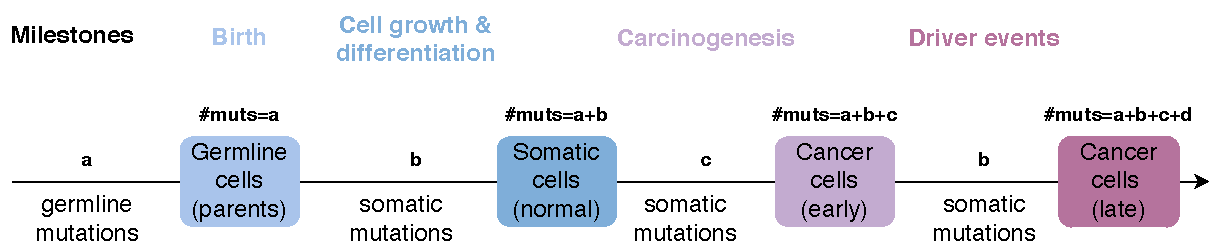
\includegraphics[scale=0.78]{graphics/drivers_demo.pdf}
    \caption{\textbf{Timeline of a carcinogenesis process.} Mutations are generally retained in the genome after each stage of carcinogenesis, even though carcinogenesis and driver events could change the phenotype of the cells. Together, all mutations available in a cancer cell make up it mutation profile. For the purpose of this project, only somatic mutations are considered because germline mutations occur prior to birth and are not the product of the environment of the differentiated cells in which cancer develop.}
    \label{fig:drivers_demo}
\end{figure}


\subsection{Significance}\label{intro:significance}
The mutation profile reflects the mechanism of mutagenesis, which offers a great opportunity to study cancer and to develop a cancer classifier that relies purely on mutation data. Being able to elucidate the mechanisms of cancer mutagenesis could potentially benefit treatments. Currently, precision medicine research focuses on targeting driver genes \citep{Mukherjee2019Genomics-GuidedCancer}. For this reason, an enhanced understanding of mutations independently of genes could perhaps expand the space for cancer therapy. \citet{Chowdhury2018PresenceNucleotides} indeed proposed to introduce the CpG motif into the genome of dividing cancer cells because this motif is very vulnerable to mutations - the rationale was to neutralise the mutation rate in important regions of the genome. Furthermore, I seek to train a \gls{classifier} that only relies on mutation data. In the long term, such a classifier could be an additional diagnostic tool to existing clinical approaches such as cytology or biopsy \citep{Stone1995Biopsy:Pitfalls}. In this era of next generation sequencing, liquid biopsies are gaining interest as a powerful non-invasive method for early cancer diagnosis because they involve screening for circulating tumour DNA in the blood rather than obtaining samples from a suspected local tissue \citep{Chen2019Next-generationDetection}. Developing a genome-based classifier model means that liquid biopsies could inform not only whether a cancer is present, but also where and what cancer is occurring at an early stage.  

\subsection{Scope}
In this project, I examined two aspects of cancer mutation profiles: (1) where mutations tend to be found in the genome (hereafter Genomic Location Effect, GLE), and (2) what base substitutions tend to be found in which genomic sequence context (hereafter Sequence Context Effect, SCE). The scope of this project is limited to point mutations, which are the most readily available type of mutations in cancer \citep{Alexandrov2020}. Additionally, since driver and passenger mutations have markedly different abundances, they should be considered separately. In this project, I focused on passenger mutations because of their abundance \citep{McFarland2014Tug-of-warProcesses}. Finally, I only investigated \glspl{sommut} as opposed to \glspl{germline_mut}, acknowledging that germline mutations could themselves be a risk factor of cancer. This is because germline mutations are present in effectively all the cells of a person, hence they are not the direct consequence of the mutagenic environment (Figure \ref{fig:drivers_demo}).

Section \ref{intro:gle} and \ref{intro:sce} of this chapter review what is known about GLE and SCE, respectively. Section \ref{intro:ml} briefly introduces the computational approaches used to study GLE and SCE, as well as how they can be used to train a machine learning classifier. Section \ref{intro:aims} summarises the aims and questions of the project. Section \ref{intro:findings} outlines the key findings.

\section{Genomic location effect (GLE)}
\label{intro:gle}
Certain regions of the genome are more prone to mutations than others, with the locations of these regions in the genome varying in different cells and cancer types \citep{Polak2015, Jiao2020}. This is suggested to result from the influence of chromatin structures on DNA accessibility, which differ in different cell types \citep{Abascal2020ExpandedGenomes}. The accessibility of DNA to transcription, mutagens and repair systems can be measured by Dnase I hypersensitivity \citep[DHS;][]{Liu2019AApplications}. In a DHS experiment, DNA is degraded by exposure to the enzyme Dnase and the degree of degradation is proportional to how accessible the DNA region is. Highly accessible DNA means open chromatin status, and vice versa. Interestingly, it has been reported that open chromatin regions are less likely to harbour mutations than closed regions \citep{Polak2015,Prendergast2007ChromatinGenome}. Given that both \gls{mutagen} exposure and DNA repair determine whether mutations occur \citep{Ripley2001Mutation}, and that DNA is less accessible to both in closed regions, the bias suggests that the repair effect is generally stronger \citep[Figure \ref{fig:chromatin_demo};][]{Teng1997ExcisionSequences, Morse2002PhotoreactivationCerevisiae}. That said, the question remains how important chromatin structure is as a determinant of the genomic location of mutations. 

\begin{figure}[h!]
    \centering
    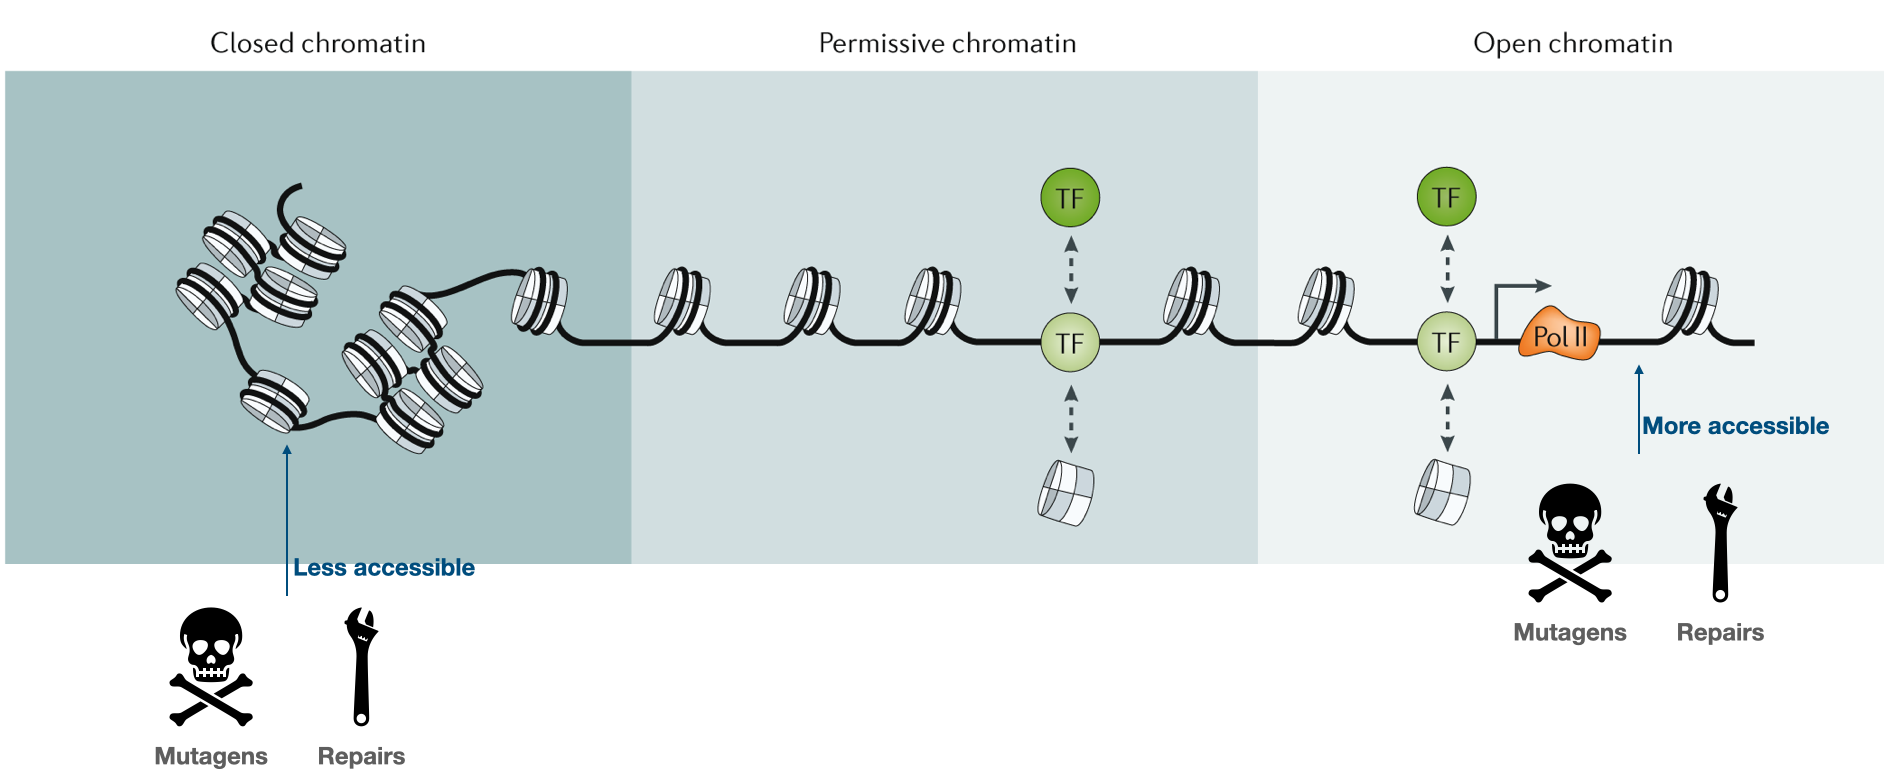
\includegraphics[scale=0.24]{graphics/chromatin_demo.png}
    \caption{\textbf{The distribution of mutations across the genome is hypothetically influenced by cell chromatin structure.} DNA in closed chromatin regions is not accessible to both mutagens and repairs, and is more prone to mutations. Different cell types have different chromatin structures as well as different repair systems, making genomic location effect (GLE) a potential factor that makes a cancer distinct from another. Figure modified from \citet{Klemm2019ChromatinEpigenome}. TF means transcription factor, Pol II means polymerase II}.
    \label{fig:chromatin_demo}
\end{figure}


Besides testing the hypothetical connection between chromatin structure and mutation location, it is equally intriguing to examine whether and how GLE can act as a distinctive characteristic of cancer mutation profiles. To represent genomic location data, the convention is to segment the genome into discrete bins, which is referred to as the bin method in this thesis \citep{Kubler2019, Salvadores2019PassengerTumors, Chalmers2017AnalysisBurden, Salvadores2020MatchingPatterns}. The bin method divides the genome into consecutive segments of 1 Mbp in length, then counts the number of mutations in each segment. However, binning imposes arbitrary boundaries to the genome and there is no biological basis for the 1 Mbp bin size. This leads to an unstable representation that is distorted when only slightly shifting the start of the bin boundaries (Figure \ref{fig:mutdistribution_demo}). 

To counteract this, my project experimented with smoothing GLE by estimating the \gls{density} at a genomic location based on the amount of data adjacent to it (details in Methods \ref{methods:bootstrap}). The smooth representation assumes no rigid boundaries to the genome, and is thus less sensitive to the above pitfall. 

\begin{figure}[h!]
  \begin{minipage}[c]{0.45\textwidth}
    \caption{
      \textbf{In theory, the smoothing approach should be more robust than the bin approach.} Both panels depict the same mutation location data for a hypothetical chromosome, with the black dots below the x-axis representing the true location of mutations. By binning the genome by convention, one counts the number of mutations in each yellow bin. The obtained GLE data is then the yellow dots on top of each bin. This binned GLE data changes when shifting the bin boundaries from panel (a) to panel (b). Mutations on the right hand side of the last bin (10$^{th}$ bin) are forcefully removed. By smoothing the genome, GLE data is the same for both panels. The smoothing method also allows inclusion of mutations outside the last bins.
    } \label{fig:mutdistribution_demo}
  \end{minipage}\hfill
  \begin{minipage}[c]{0.52\textwidth}
    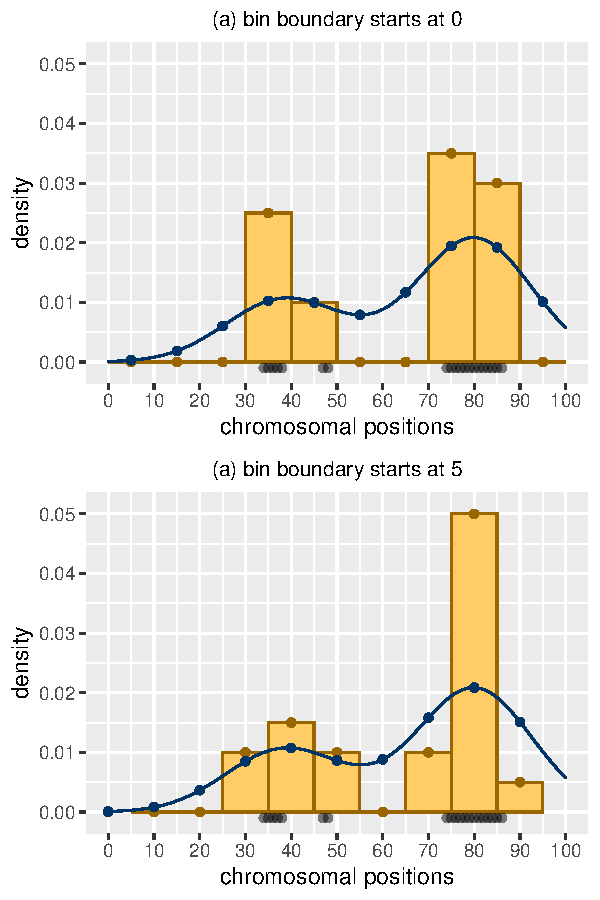
\includegraphics[width=\textwidth]{graphics/mutdistribution_demo.pdf}
  \end{minipage}
\end{figure}


\section{Sequence context effect (SCE)}
\label{intro:sce}

Each cancer develops under the influence of different mutagenic processes, giving rise to diverse mutation compositions. These processes include, but are not limited to UV light \citep[known to drive skin melanoma;][]{Mohania2017}, the intrinsic cellular APOBEC deaminase activity \citep[\textit{e.g.} in B cells;][]{Kuppers2005MechanismsPathogenesis} and defective DNA repair \citep[\textit{e.g.} mutated \textit{BRCA} genes in breast cancer;][]{Navasardyan2021YY1TNBC}. \citet{Alexandrov2013, Alexandrov2020} showed that some processes were associated with certain mutation signatures. For instance, the signature SBS4, where there is an excess of C$\rightarrow$A substitutions in the context of C[C$\rightarrow$A]A and C[C$\rightarrow$A]C over any other mutations, was only detected in tobacco smoke linked cancers such as liver hepatocellular carcinoma, lung adenocarcinoma and lung squamous cell carcinoma \citep{Alexandrov2020}. As such, similar to GLE, SCE is also an important characteristic of the cancer mutation profile. 

The analysis of SCE was motivated by the statistical associations between the base substitutions and the \glspl{base} next to them \citep{Zhu2017}. A well known example is that the C$\rightarrow$T mutations tend to occur in the [C$\rightarrow$T]G context due to the high binding affinity of methyltransferase to the CpG motif \citep[Figure \ref{fig:motif_demo};][]{Cooper2010}. Methyltransferase methylates CpG, making it very vulnerable to mutations. There are two potential flaws in the standard way of representing SCE. First, while it is common practice to analyse mutation compositions in the 3-mer (3 position) context, there is evidence that bases beyond 3-mer were also associated with mutations \citep{Zhu2017,Zhu2020}. Second, base substitutions are generally assumed to be strand symmetric, meaning G$\rightarrow$A and its reverse complementary counterpart C$\rightarrow$T are counted as the same category \citep[Figure \ref{fig:motif_symmetric_demo};][]{Alexandrov2013, Jiao2020}. However, analyses in skin melanoma advocated different mutation patterns between two DNA strands, suggesting that the strand symmetric representation could be missing information \citep{Zhu2017}. Accordingly, I seek to explore the information content available in different sequence context sizes, particularly the outer positions of the 5-mer context (positions -2 and +2 with respect to the substitutions); as well as the effect of strand symmetry/asymmetry in representing SCE.

\begin{figure}[h!]
    \centering
    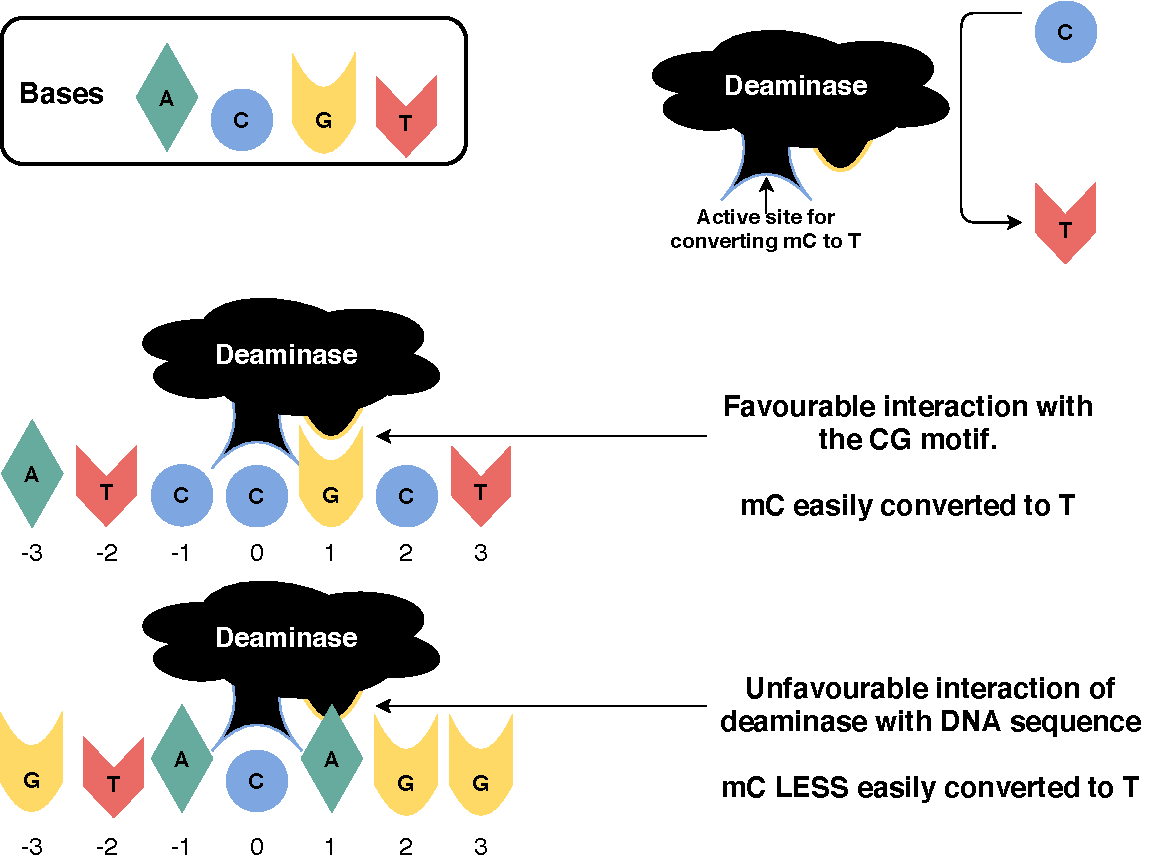
\includegraphics[scale=0.78]{graphics/motif_demo.pdf}
    \caption{\textbf{Mutations are closely linked with the bases next to them}. The schematic diagram depicts an example of hypothetical scenarios that could explain why this is the case. Here, a deaminase protein, which converts methylated C into T, interacts with DNA such that certain sequence contexts make the conversion more feasible than others. While many publications focus on the 3-mer context of mutations (pos -1, 0 and 1), which includes the base change and two bases immediately next to it, evidence shows that bases outside the 3-mer could still be influential. Part of this project seeks to explore the information content available in larger sequence contexts than 3-mers.}
    \label{fig:motif_demo}
\end{figure}

\begin{figure}[h!]
    \centering
    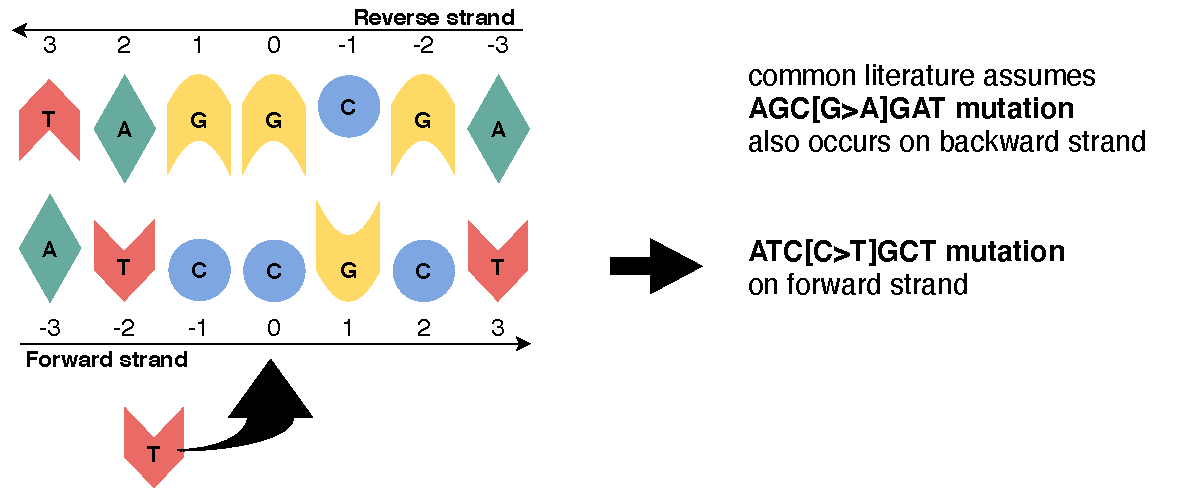
\includegraphics[scale=0.78]{graphics/motif_symmetric_demo.pdf}
\caption{}
    % \caption{\textbf{It is common practice to assume strand symmetry when analysing mutations.} In this example, AGC[G$\rightarrow$A]GAT and ATC[C$\rightarrow$G]GCT mutations on the reverse complementary strand are counted as the same category. However, observations supporting strand asymmetry have been reported. This project explores the effect of the strand symmetric \textit{v.s.} strand asymmetric assumption.}
    \label{fig:motif_symmetric_demo}
\end{figure}


\section{Computational approaches to study GLE and SCE}
\label{intro:ml}

The technical part of this project had two equally important aspects: statistics and computing, simultaneously serving two purposes: data analysis and method development. The statistical aspect was to understand and manipulate the data for answering the questions of interest. The experimental design and the choice of the statistical analyses were guided by our knowledge of the properties of both the statistical tools and the data investigated. The computational aspect of the project was a means to execute the experimental design. It is important for computational tools accurately carry out what had been outlined in the experimental design, and to produce the same outcome if executed multiple times. As a result, throughout the project, my code was thoroughly tested and all changes were tracked (details in Methods \ref{methods:code}). 

The release of the \gls{pcawg} project \citep{Campbell2020}, with whole genomic sequencing data for 2605 primary tumours of 38 cancer types, has made studying cancer genomics and developing cancer classification models on a large scale feasible. I analysed the data on two levels. First, data was investigated on the whole disease level (\gls{gle} in Chapter \ref{gle}; \gls{sce} in Chapter \ref{sce}). This means that for each cancer, mutations from all donors of that cancer were considered as a whole. This makes understanding the mutagenesis process easier as it magnifies the signals in the data provided they really exist. Second, Chapter \ref{ml} trialled different measures and data representations to train the classifiers on the individual donor level. The idea is that the more accurate the classifier, the better the assumptions imposed by its data representations could capture the nature of the data. The long term goal is to be able to apply the model to unseen data, such as the tumour genome of a new cancer patient. Thus, the analyses on two levels were complementary and can be used to verify each other. Whereas whole disease analysis explored how and why a potential factor might be important, individual scale was a direct measure of how informative that factor was.  

\section{Aims and questions}
\label{intro:aims}
\begin{enumerate}
    \item To evaluate the influence of chromatin structure on genomic location effect (GLE) and the degree at which GLE can discriminate cancers (Chapter \ref{gle})
    \begin{itemize}
        \item Are mutations significantly biased towards closed or open regions?
        \item Is the bias uniform for all cancers?
        \item Is the proposed smooth representation better at extracting information than the conventional bin approach?
    \end{itemize}
    \item To understand how sequence context effect (SCE) is characteristic of cancers (Chapter \ref{sce})
    \begin{itemize}
        \item Can the base substitutions discriminate cancers?
        \item Are the flanking bases informative? Is there any advantage in studying bases at outer positions such as positions -2 and +2?
        \item Are mutations, including base substitutions and flanking bases, strand symmetric?
    \end{itemize}
    \item To train a classifier that accurately predicts cancers for individual donors (Chapter \ref{ml})
    \begin{itemize}
        \item Do the proposed methods for GLE and SCE outperform those normally used?
        \item Do the representations used by the best classifier match those identified by whole disease analyses?
        \item Does combining SCE and GLE result in further accuracy improvement than each factor alone?
    \end{itemize}
\end{enumerate}

\section{Key findings}
\label{intro:findings}
Overall, the project shows that both GLE and SCE are important characteristics of a cancer \gls{mut_profile}, manifesting in three aspects. First, Chapter \ref{gle} shows that mutations generally tended to occur in closed chromatin regions, but the degree of bias varied between cancers. This suggests that chromatin structure has an important influence on GLE, but it is not the single determinant of GLE. Regardless of the driving forces, GLE was found to be characteristic of cancers, particularly when the smoothing representation was used. Second, both components of SCE, the base substitutions and their sequence contexts were characteristic of cancers (Chapter \ref{sce}). Information was more abundant closer to the substitutions (3-mer), but the outer bases were also very informative. Additionally, there was more information in \glspl{transition} than in \glspl{transversion} for both base substitutions and their flanking bases in Chapter \ref{ml}, with evidence of strand symmetry. When recruited to train classifiers, smoothing GLE provided a higher predictive power than binning. Regarding SCE, incorporating the immediate neighbours within the 3-mer neighbourhood improved accuracy over the base changes alone. In addition, while information was detected in the outer bases of the 5-mer sequence context, incorporating this information into the classifier was not supported. Finally, even though GLE and SCE were expected to be separate sources of information, SCE was the predominating contributor of the combined classifier. To be exact, there was no improvement in predictive power in the combined classifier compared to the SCE classifier when using the proposed representations.
